\section{Конструкторская часть}

\subsection{Проектирование БД}

База данных должна хранить представленные в таблице \ref{tab:data} данные. Исходя из этого, в проектируемой базе данных можно выделить следующие таблицы:
\begin{itemize}
	\item таблица с реп. базами (rehbase);
	\item таблица с комнатами реп. баз (room);
	\item таблица с оборудованием в комнатах (equipment);
	\item таблица с аккаунтами пользователей (account);
	\item таблица с забронированными репетициями (rehearsal).
\end{itemize}

Таблица rehbase должна содержать информацию о:
\begin{itemize}
	\item id – идентификатор реп. базы (PK);
	\item name – название реп. базы (text);
	\item address – адрес реп. базы (text);
	\item phone – номер телефона для связи (text);
	\item mail – электронная почта для связи (text);
	\item ownerid – id владельца реп. базы (связь с таблицей account) (FK, один-ко-многим).
\end{itemize}

Таблица room должна содержать информацию о:
\begin{itemize}
	\item id – идентификатор комнаты (PK);
	\item name – название комнаты (text);
	\item type – тип комнаты (text);
	\item area – площадь комнаты (integer);
	\item cost – стоимость репетиции в этой комнате за 3 часа (integer);
	\item baseid – id реп. базы, которой принадлежит комната (связь с таблицей rehbase) (FK, один-ко-многим).
\end{itemize}

Таблица equipment должна содержать информацию о:
\begin{itemize}
	\item id – идентификатор оборудования (PK);
	\item type – тип оборудования (text);
	\item brand – фирма оборудования (text);
	\item amount – количество оборудования такого типа в соответствующей комнате (integer);
	\item roomid – id комнаты, в которой находится это оборудование (связь с таблицей room) (FK, один-ко-многим).
\end{itemize}

Таблица account должна содержать информацию о:
\begin{itemize}
	\item id – идентификатор пользователя (PK);
	\item fio – ФИО пользователя (text);
	\item phone – номер телефона пользователя (text);
	\item mail – электронная почта пользователя (text);
	\item password – пароль от аккаунта (text);
	\item type – тип пользователя (text).
\end{itemize}

Таблица rehearsal должна содержать информацию о:
\begin{itemize}
	\item id – идентификатор репетиции (PK);
	\item rehdate – дата и время репетиции (timestamp);
	\item musicianid – id музыканта, забронировавшего репетицию (связь с таблицей account) (FK, один-ко-многим);
	\item roomid – id комнаты, в которой забронирована репетиция (связь с таблицей room) (FK, один-ко-многим).
\end{itemize}

\begin{figure}[h!]
	\begin{center}
		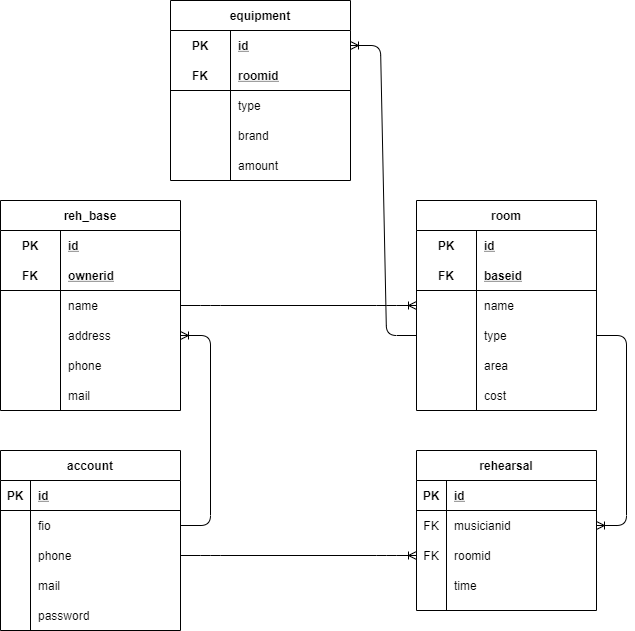
\includegraphics[scale=0.5]{inc/img/ER_DB.png}
	\end{center}
	\captionsetup{justification=centering}
	\caption{ER диаграмма проектируемой БД}
	\label{img:er}
\end{figure}

\newpage

\subsection{Требования к программе}

Разрабатываемое ПО должно предоставлять следующие возможности:
\begin{itemize}
	\item регистрация нового пользователя;
	\item авторизация пользователя;
	\item вывод списка комнат, доступных для бронирования;
	\item вывод подробной информации о каждой комнате;
	\item бронь комнаты на соответствующее время;
	\item отмена брони;
	\item вывод уже забронированных (будущих) репетиций;
	\item вывод зарегистрированных реп. баз для данного аккаунта;
	\item регистрация новой реп. базы;
	\item добавление комнаты в зарегистрированную реп. базу;
	\item добавление оборудования в соответствующую комнату;
	\item вывод всех будущих репетиций на соответствующей реп. базе;
	\item удаление реп. базы;
	\item поиск по имени реп. базы;
	\item поиск по дате и времени репетиции.
\end{itemize}

Ограничения, в рамках которых будет работать программа:
\begin{itemize}
	\item аккаунт нельзя удалить;
	\item нельзя зарегистрироваться стандартным способом в качестве администратора (администраторы добавляются «вручную» на уровне БД);
	\item для обновления информации нужно закрыть соответствующее окно и снова его открыть;
	\item для выхода из аккаунта нужно закрыть окно;
	\item пароль от аккаунта хранится в БД в обычном виде, без шифрования;
	\item календарь для бронирования репетиций не предоставляется.
\end{itemize}

\subsection{Структура ПО}

Всё проектируемое ПО можно разделить на две основные части:
\begin{itemize}
	\item frontend (часть приложения, с которой непосредственно взаимодействует пользователь, отображение данных);
	\item backend (взаимодействие с базой данных).
\end{itemize}

Структура frontend части в свою очередь будет основана на паттерне MVC (Model, View, Controller).

Таким образом, проект будет разделён на несколько файлов:
\begin{itemize}
	\item connect – взаимодействие непосредственно с БД;
	\item gui – здесь будут находиться модели и контроллеры frontend части;
	\item отдельные файлы для каждого окна итогового приложения, предоставляющие интерфейс пользователю (т. е. отвечающие за view часть).
\end{itemize}

Файл connect будет состоять из набора следующих функций:
\begin{itemize}
	\item connect\_* – для подключения к БД с соответствующей ролью;
	\item функции для формирования и посылки запросов к БД.
\end{itemize}

Файл gui в свою очередь будет состоять из набора классов, каждый из которых будет соответствовать определённому окну приложения.

На рисунке \ref{img:classes} представлена диаграмма классов разрабатываемого приложения.

\begin{figure}[h!]
	\begin{center}
		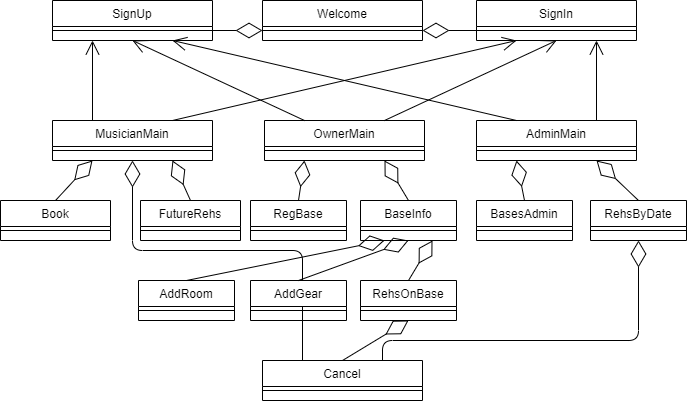
\includegraphics[scale=0.6]{inc/img/Classes.png}
	\end{center}
	\captionsetup{justification=centering}
	\caption{Диаграмма классов}
	\label{img:classes}
\end{figure}

\subsection{Способы и этапы тестирования}

Для проверки работоспособности ПО будет применяться функциональное тестирование.

Тестирование ПО будет разделено на следующие этапы:
\begin{itemize}
	\item регистрация нового пользователя (как музыканта, так и владельца);
	\item попытка зарегистрироваться ещё раз с той же почтой;
	\item попытка авторизоваться с неправильной почтой или паролем;
	\item авторизация в качестве музыканта;
	\begin{itemize}
		\item бронирование репетиции;
		\item попытка забронировать репетицию в уже забронированной на это время комнате;
		\item просмотр своих будущих репетиций;
		\item отмена брони;
		\item попытка забронировать репетицию «в прошлом»;
	\end{itemize}
	\item авторизация в качестве владельца;
	\begin{itemize}
		\item регистрация новой реп. базы;
		\item попытка зарегистрировать уже существующую реп. базу (с той же почтой либо с тем же названием и адресом);
		\item добавление комнаты в реп. базу;
		\item попытка добавить уже существующую комнату (с тем же названием);
		\item добавление оборудования в комнату;
		\item попытка добавить оборудование в несуществующую комнату;
		\item попытка повторно добавить то же самое оборудование в ту же самую комнату;
		\item просмотр предстоящих репетиций на соответствующей реп. базе;
		\item удаление реп. базы;
	\end{itemize}
	\item авторизация в качестве администратора;
	\begin{itemize}
		\item поиск реп. баз по названию (успешный);
		\item попытка найти несуществующую реп. базу;
		\item поиск репетиций по дате (успешный);
		\item попытка найти несуществующую репетицию.
	\end{itemize}
\end{itemize}

\subsection*{Выводы}

На основе теоретических данных, полученных в аналитическом разделе, были спроектированы база данных и приложение. А также были приведены: требования к программе, способы и этапы тестирования и диаграмма классов.

